\section{Results}
\label{sec:results}

\subsection{Ranking quality does not predict the false-alarm budget}
\label{sec:res_zero}

% AUTO-GENERATED by tools/paper_tables.py -- do not edit by hand
\begin{table}[t]
\centering
\small
\setlength{\tabcolsep}{4pt}
\caption{Ranking quality does not predict whether the false-alarm budget is kept. Left: video AUC. Right: false-positive rate on authentic target videos when the alert threshold is the $95$th percentile of FF++ validation reals (nominal budget $\alpha=0.05$). Mean$\pm$sd over training seeds; bold marks rates above $2\alpha$. $^\dagger$Published checkpoint, single run.}
\label{tab:ranking_vs_budget}
\resizebox{\linewidth}{!}{%
\begin{tabular}{lc ccc ccc}
\toprule
 & & \multicolumn{3}{c}{Video AUC $\uparrow$} & \multicolumn{3}{c}{FPR at source threshold ($\alpha=0.05$)} \\
\cmidrule(lr){3-5}\cmidrule(lr){6-8}
Detector & Seeds & Celeb-DF & DFD & FakeAVCeleb & Celeb-DF & DFD & FakeAVCeleb \\
\midrule
GenD (official)$^\dagger$ & 1 & 0.933 & 0.884 & 0.974 & \textbf{0.157} & \textbf{0.193} & 0.084 \\
GenD-style (ours) & 3 & 0.829$\pm$0.002 & 0.866$\pm$0.003 & 0.891$\pm$0.002 & 0.017$\pm$0.000 & 0.011$\pm$0.002 & \textbf{0.112$\pm$0.014} \\
S-MSDT-S & 3 & 0.883$\pm$0.001 & 0.877$\pm$0.010 & 0.944$\pm$0.004 & 0.058$\pm$0.009 & 0.053$\pm$0.008 & 0.045$\pm$0.026 \\
S-MSDT-ST & 3 & 0.870$\pm$0.008 & 0.862$\pm$0.007 & 0.939$\pm$0.008 & 0.084$\pm$0.010 & 0.096$\pm$0.010 & 0.051$\pm$0.011 \\
S-MSDT-Full & 3 & 0.888$\pm$0.010 & 0.845$\pm$0.013 & 0.945$\pm$0.001 & \textbf{0.122$\pm$0.034} & \textbf{0.134$\pm$0.061} & 0.092$\pm$0.023 \\
\bottomrule
\end{tabular}}
\end{table}


Table~\ref{tab:ranking_vs_budget} sets AUC beside the false-positive rate obtained when the alert threshold is the $95$th percentile of FF++ validation reals. Three observations stand out.

First, the published GenD checkpoint has the best AUC on every target, and the worst budget transfer on Celeb-DF ($0.157$, $3.1\times$ the budget) and DFD ($0.193$, $3.9\times$). Good ranking and a good operating point are separate properties. Second, the same detector can be over budget on one target and under it on another. GenD-style (ours) is far below budget on Celeb-DF and DFD ($0.017$ and $0.011$), which wastes recall, and over $2\alpha$ on FakeAVCeleb ($0.112$). Third, the effect varies with the training seed: S-MSDT-Full ranges from $0.090$ to $0.157$ on Celeb-DF and from $0.066$ to $0.181$ on DFD across its three seeds. A deployer who validated one seed would not know what the next retraining does to the budget. Only S-MSDT-S stays within a factor of $1.5$ of the budget on all three targets, and we have no evidence that this holds beyond these datasets.

The registered test H4a, which asked whether ST and Full exceed $2\alpha$ on unseen data, is undetermined because its confirmatory seeds were not trained (Table~\ref{tab:hyp}). Descriptively, the lower end of the $95\%$ interval of the FPR exceeds $2\alpha$ in 9 of the 78 detector--target--budget rows of the audit; four of these are the published GenD checkpoint (Appendix~\ref{app:extra}).

\subsection{Label-free repairs do not restore the budget}
\label{sec:res_labelfree}

% AUTO-GENERATED by tools/paper_tables.py -- do not edit by hand
\begin{table}[t]
\centering
\small
\caption{Label-free repair with a two-component Gaussian mixture fitted to unlabelled target scores ($\alpha=0.05$). On FakeAVCeleb ($83\%$ fakes) the mixture places the threshold where it detects few fakes. Mean over seeds.}
\label{tab:label_free}
\begin{tabular}{l cc cc}
\toprule
 & \multicolumn{2}{c}{Celeb-DF} & \multicolumn{2}{c}{FakeAVCeleb} \\
\cmidrule(lr){2-3}\cmidrule(lr){4-5}
Detector & FPR & TPR & FPR & TPR \\
\midrule
GenD (official)$^\dagger$ & 0.022 & 0.629 & 0.004 & 0.540 \\
GenD-style (ours) & 0.157 & 0.663 & 0.009 & 0.328 \\
S-MSDT-S & 0.041 & 0.503 & 0.000 & 0.506 \\
S-MSDT-ST & 0.109 & 0.598 & 0.000 & 0.000 \\
S-MSDT-Full & 0.000 & 0.154 & 0.000 & 0.000 \\
\bottomrule
\end{tabular}
\end{table}


A deployer without target labels might fit a two-component Gaussian mixture to the unlabelled target scores and read off the threshold for the authentic component. Table~\ref{tab:label_free} shows two failure modes. On Celeb-DF, where about two thirds of videos are fake, the mixture breaks the budget for GenD-style ($0.157$) and S-MSDT-ST ($0.109$). On FakeAVCeleb, where $83\%$ are fake, it keeps the FPR near zero by placing the threshold where few fakes are detected: TPR is $0.33$--$0.54$ for three detectors and $0$ for S-MSDT-ST and S-MSDT-Full, whose fits are degenerate in every seed. H5, which required the mixture to halve the FPR error of the source threshold under prior stress, is falsified for both mixture variants.

Test-time adaptation of the LayerNorm parameters by entropy minimization \citep{wang2021tent} collapses when run online over the test stream: on Celeb-DF, AUC falls from $0.888$ to $0.339$ and the share of videos predicted fake falls to $6.6\%$ against a true $65.6\%$; DFD behaves the same way ($0.858\to0.239$). Our clip-consistency objective slows the drift but still collapses ($0.541$). Episodic adaptation, which resets the parameters after every batch, avoids collapse but leaves AUC unchanged to four decimals, so it cannot lower the error. H3b and H6 are falsified. EM prior correction \citep{saerens2002adjusting} misestimates the fake prior by $0.07$ to $0.17$ on average and does not lower the frozen-threshold HTER at any prior we tried, so H3a is falsified; as noted in the decision log, HTER averages the two error rates and is insensitive to the prior, so H3a was poorly posed. Full tables are in Appendix~\ref{app:extra}.

\subsection{Twenty authentic identities restore the budget}
\label{sec:res_realshot}

% AUTO-GENERATED by tools/paper_tables.py -- do not edit by hand
\begin{table}[t]
\centering
\small
\setlength{\tabcolsep}{3.5pt}
\caption{Real-shot calibration on FakeAVCeleb with $n=20$ authentic identities ($\alpha=0.05$, 500 identity-disjoint draws per run, evaluation on the remaining $479$ identities). Mean over seeds with (min--max). ``Retained'' is conformal TPR divided by the oracle TPR obtained with test-set reals. The expected conformal FPR at $n=20$ is $1/21=0.048$.}
\label{tab:real_shot}
\resizebox{\linewidth}{!}{%
\begin{tabular}{l c cc cc c}
\toprule
 & Source & \multicolumn{2}{c}{Naive quantile} & \multicolumn{2}{c}{Conformal (ours)} & \\
\cmidrule(lr){3-4}\cmidrule(lr){5-6}
Detector & FPR & FPR & $P(\mathrm{FPR}>2\alpha)$ & FPR & $P(\mathrm{FPR}>2\alpha)$ & Retained TPR \\
\midrule
GenD (official)$^\dagger$ & 0.084 & 0.090 & 0.38 & 0.046 & 0.11 & 92.7\% \\
GenD-style (ours) & 0.112 (0.096--0.122) & 0.086 (0.086--0.087) & 0.32 (0.31--0.33) & 0.045 (0.045--0.046) & 0.10 (0.09--0.10) & 84.2\% (83.5--85.2) \\
S-MSDT-S & 0.045 (0.022--0.074) & 0.088 (0.087--0.089) & 0.36 (0.35--0.37) & 0.046 (0.045--0.047) & 0.12 (0.10--0.13) & 96.3\% (95.4--96.8) \\
S-MSDT-ST & 0.051 (0.038--0.058) & 0.088 (0.085--0.090) & 0.35 (0.32--0.39) & 0.046 (0.046--0.047) & 0.12 (0.11--0.13) & 93.7\% (93.3--94.0) \\
S-MSDT-Full & 0.092 (0.066--0.108) & 0.087 (0.087--0.087) & 0.36 (0.35--0.38) & 0.044 (0.044--0.045) & 0.11 (0.11--0.12) & 94.1\% (92.2--95.1) \\
\bottomrule
\end{tabular}}
\end{table}


\begin{figure}[t]
\centering
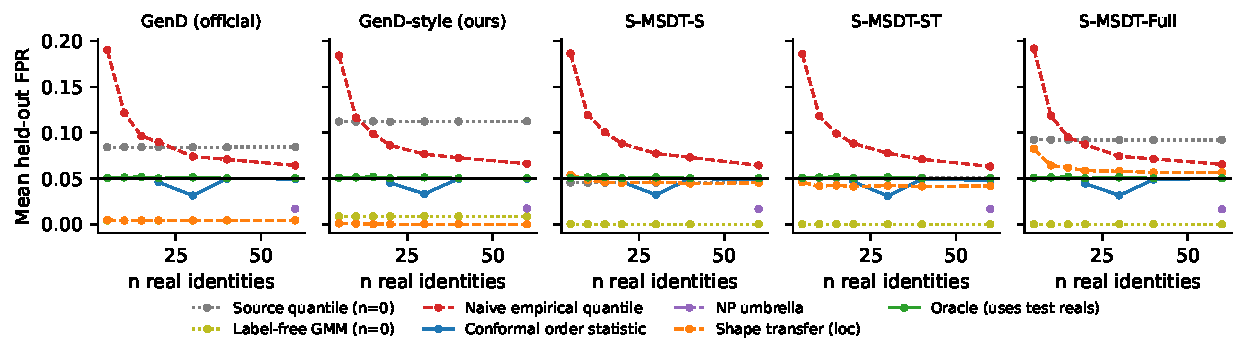
\includegraphics[width=\linewidth]{figures/confirm/fig2_real_shot_fpr.pdf}
\caption{Mean false-positive rate on held-out authentic FakeAVCeleb identities as a function of the number $n$ of target reals used for calibration ($\alpha=0.05$, solid black line; 500 draws per point, averaged over seeds). The conformal rule abstains below $n=19$; its dip at $n=30$ is the conservative value $(n+1-k)/(n+1)=0.032$ predicted between sweet spots. The naive quantile overshoots at small $n$; the source threshold and the label-free mixture do not depend on $n$.}
\label{fig:real_shot_fpr}
\end{figure}

Table~\ref{tab:real_shot} and Figure~\ref{fig:real_shot_fpr} give the confirmatory result on FakeAVCeleb. With $n=20$ authentic identities, the conformal threshold gives a mean FPR between $0.044$ and $0.047$ in all 13 runs, against the expected $1/21=0.048$, and keeps between $83.5\%$ and $96.8\%$ of oracle recall (mean $92.1\%$). Both conditions of H7b-v2 hold in every run, so it is supported. The empirical quantile of the same 20 videos, which differs only by using $n$ in place of $n+1$, gives $0.085$--$0.090$ and exceeds $2\alpha$ in $31$--$39\%$ of draws; H7c-v2 is supported. The finite-sample correction is the whole difference: it costs one order statistic and halves the false-alarm rate.

The conformal rule is valid on average, not in every draw: its audited rate exceeds $2\alpha$ in $9$--$13\%$ of draws at $n=20$. That is close to the $0.122$ that Proposition~\ref{prop:bb} predicts for $m=479$ (Table~\ref{tab:planner}). The next section tests this prediction systematically.

H7a-v2, which asked whether every zero-shot threshold has some run with $P(\mathrm{FPR}>2\alpha)>0.2$, is not supported. The source threshold meets this condition, but the mixture threshold never exceeds $2\alpha$ on FakeAVCeleb because, as shown above, it fails by losing recall instead. On the Celeb-DF development data the conformal rule behaves the same way within each source of authentic video (Appendix~\ref{app:extra}).

\subsection{Pre-registered test of the budget certificate (H8)}
\label{sec:res_h8}

% AUTO-GENERATED by tools/paper_tables.py -- do not edit by hand
\begin{table}[t]
\centering
\small
\setlength{\tabcolsep}{4pt}
\caption{Pre-registered H8 audit: 13 detectors $\times$ 2 target datasets $\times$ 5 calibration sizes $=130$ cells, $R=1{,}000$ identity-disjoint draws per cell. ``Pred.'' is the closed-form Beta-Binomial probability that the held-out FPR exceeds $2\alpha$; ``Obs.'' is the observed frequency, averaged over the 13 detectors. Criterion (i): observed frequency inside the $99\%$ binomial interval of the prediction. Criterion (ii): mean FPR $\le\alpha+2\,\mathrm{SE}_{\mathrm{MC}}$. H8 required (i) in $\ge 90\%$ of cells and (ii) in every cell.}
\label{tab:h8}
\begin{tabular}{l cc c cc c cc c}
\toprule
 & & & & \multicolumn{3}{c}{$P(\mathrm{FPR}_{\mathrm{eval}}>2\alpha)$} & \multicolumn{2}{c}{Mean FPR} & \\
\cmidrule(lr){5-7}\cmidrule(lr){8-9}
Target & $\alpha$ & $n$ & $m$ & Pred. & Obs. & (i) pass & Value & (ii) pass & Retained TPR \\
\midrule
FakeAVCeleb & 0.05 & 19 & 480 & 0.135 & 0.143 & 13/13 & 0.0514 & 11/13 & 93.3\% \\
FakeAVCeleb & 0.05 & 39 & 460 & 0.091 & 0.090 & 13/13 & 0.0503 & 13/13 & 96.4\% \\
FakeAVCeleb & 0.05 & 59 & 440 & 0.063 & 0.066 & 13/13 & 0.0505 & 11/13 & 97.7\% \\
FakeAVCeleb & 0.10 & 9 & 490 & 0.134 & 0.139 & 13/13 & 0.1022 & 12/13 & 94.4\% \\
FakeAVCeleb & 0.10 & 29 & 470 & 0.055 & 0.055 & 13/13 & 0.1012 & 12/13 & 98.4\% \\
\midrule
Celeb-DF & 0.05 & 19 & 102 & 0.140 & 0.130 & 13/13 & 0.0489 & 13/13 & 85.6\% \\
Celeb-DF & 0.05 & 39 & 82 & 0.107 & 0.107 & 13/13 & 0.0504 & 13/13 & 90.9\% \\
Celeb-DF & 0.05 & 59 & 62 & 0.094 & 0.093 & 13/13 & 0.0503 & 13/13 & 91.7\% \\
Celeb-DF & 0.10 & 9 & 112 & 0.139 & 0.136 & 13/13 & 0.0983 & 13/13 & 88.1\% \\
Celeb-DF & 0.10 & 29 & 92 & 0.071 & 0.074 & 13/13 & 0.0993 & 13/13 & 95.2\% \\
\bottomrule
\end{tabular}
\end{table}


\begin{figure}[t]
\centering
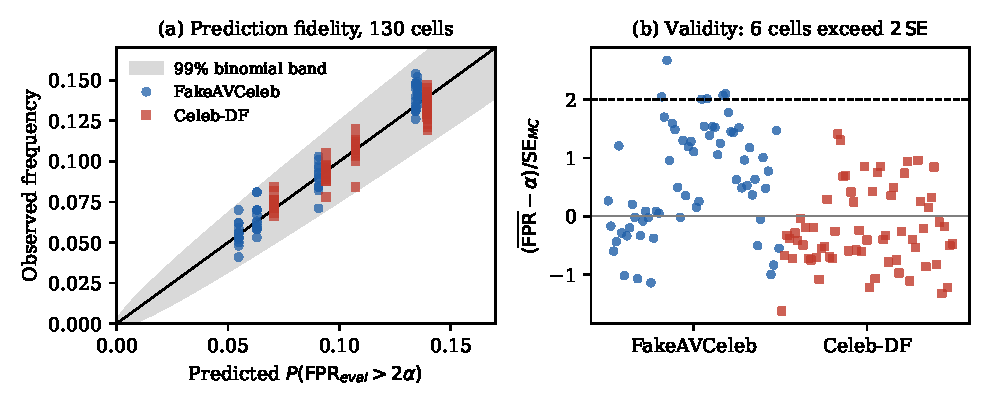
\includegraphics[width=\linewidth]{figures/fig6_h8_audit.pdf}
\caption{H8 audit over 130 cells. (a) Observed frequency of an audited FPR above $2\alpha$ against the closed-form prediction of \eqref{eq:pviol}; the grey band is the $99\%$ binomial interval for $R=1{,}000$ draws. All 130 cells lie inside it. (b) Excess of the mean FPR over $\alpha$ in Monte Carlo standard errors; six FakeAVCeleb cells lie above the registered limit of $2$.}
\label{fig:h8}
\end{figure}

H8 tests Proposition~\ref{prop:bb} across 13 detectors, both external targets and the five sweet-spot pairs $(\alpha,n)$, with $1{,}000$ draws per cell (Table~\ref{tab:h8}, Figure~\ref{fig:h8}). It was registered as supported only if (i) the observed exceedance frequency lies inside the $99\%$ binomial interval of the prediction in at least $90\%$ of cells, and (ii) the mean FPR is at most $\alpha+2\,\mathrm{SE}_{\mathrm{MC}}$ in every cell.

Criterion (i) holds in all 130 cells. The prediction tracks the observation across a range of $0.055$ to $0.143$, including the dependence on $m$: at $n=39$, the formula gives $0.091$ for FakeAVCeleb ($m=460$) and $0.107$ for Celeb-DF ($m=82$), and the observed frequencies are $0.090$ and $0.107$.

Criterion (ii) fails in 6 of 130 cells, all on FakeAVCeleb and all for S-MSDT-S seed 1 or S-MSDT-ST seeds 1--2 (Appendix~\ref{app:extra}, Table~\ref{tab:appx_h8_fail}). Their mean FPR exceeds $\alpha$ by $0.0020$ to $0.0062$, which is $2.0$ to $2.7$ standard errors. H8 is therefore \textbf{falsified as registered}.

\paragraph{Post-hoc analysis (not registered).}
Criterion (ii) was too strict for the question it was meant to answer. At the sweet spots Proposition~\ref{prop:bb} gives $\mathbb{E}[X/m]=\alpha$ exactly, so a cell's mean FPR differs from $\alpha$ only by Monte Carlo error. Each cell then exceeds $\alpha+2\,\mathrm{SE}$ with probability $0.023$, and requiring all 130 cells to pass fails with probability $1-0.977^{130}\approx0.95$ even if the law is exact and the cells are independent; about $3$ failures are expected. The cells are also not independent: the registered run seeds every cell with the same value, so all 13 detectors at a given target and $(\alpha,n)$ are evaluated on the same 1{,}000 splits. This is visible in Figure~\ref{fig:h8}(b), where the FakeAVCeleb cells are shifted upwards together. Re-running the evaluation with three other seeds removes the shift (mean standardized excess on FakeAVCeleb $-0.22$ to $-0.43$, against $+0.63$ with the registered seed) and gives 1, 3 and 3 failing cells out of 130 (Appendix~\ref{app:extra}, Table~\ref{tab:appx_h8_reseed}). Criterion (ii) fails under every seed we tried, as the calculation above predicts. We read this as evidence that the six failures reflect shared Monte Carlo noise rather than a miscalibrated law. This reading was not registered, and the registered verdict stands. A better registered test would control the family-wise error over cells, or test the mean excess pooled over cells with independent draws per cell.

\subsection{Extra head capacity does not change the picture}
\label{sec:res_capacity}

% AUTO-GENERATED by tools/paper_tables.py -- do not edit by hand
\begin{table}[t]
\centering
\small
\setlength{\tabcolsep}{4pt}
\caption{Hypothesis H1 on FakeAVCeleb (991 identity clusters, paired cluster bootstrap, $10{,}000$ resamples, equivalence margin $\delta=0.01$). The two confirmatory comparisons use Bonferroni-adjusted $97.5\%$ intervals; the others are exploratory $95\%$ intervals. AUCs pool the scores of all seeds.}
\label{tab:h1}
\begin{tabular}{l c cc c c c}
\toprule
Comparison (A $-$ B) & Role & AUC(A) & AUC(B) & $\Delta$AUC & Interval & Decision \\
\midrule
S-MSDT-ST $-$ S-MSDT-S & confirmatory & 0.9392 & 0.9437 & -0.0045 & [-0.0096, +0.0006] & equivalent \\
S-MSDT-Full $-$ S-MSDT-S & confirmatory & 0.9449 & 0.9437 & +0.0012 & [-0.0050, +0.0073] & equivalent \\
S-MSDT-S $-$ GenD-style (ours) & exploratory & 0.9437 & 0.8907 & +0.0530 & [+0.0398, +0.0668] & better \\
S-MSDT-S $-$ GenD (official)$^\dagger$ & exploratory & 0.9437 & 0.9745 & -0.0308 & [-0.0391, -0.0227] & worse \\
\bottomrule
\end{tabular}
\end{table}


The detectors we trained let us ask whether a larger head would solve the problem instead. On FakeAVCeleb, adding spatio-temporal attention (ST, $11\times$ the trainable parameters of S) or the residual stream and evidence readout (Full, $12\times$) changes pooled AUC by $-0.0045$ and $+0.0012$, and both $97.5\%$ intervals lie inside $\pm0.01$ (Table~\ref{tab:h1}). On Celeb-DF the intervals are too wide to decide, and on the development set DFD, Full is worse than S ($-0.033$; Appendix~\ref{app:extra}). The registered H1 test is undetermined because its confirmatory seeds were not trained, and the seed-to-seed standard deviation of ST on FakeAVCeleb ($0.008$) is close to the margin, so we report this as descriptive. Capacity also does not help the budget: Full has the largest source-threshold inflation of the detectors we trained (Table~\ref{tab:ranking_vs_budget}).

S-MSDT-S outperforms our GenD-style model by $0.053$ AUC on FakeAVCeleb. Because the two differ in both head and training recipe, we cannot attribute this gap to either. The published GenD checkpoint is better than S-MSDT-S by $0.031$; it was trained on a different recipe and is not a controlled comparison.
